% Chapter 5

\chapter{Experiments and Results} % Main chapter title

\label{Chapter5} % For referencing the chapter elsewhere, use \ref{Chapter5}

% This is for the header on each page - perhaps a shortened title
\lhead{Chapter 5. \emph{Experiments and Results}}

% Quotation
``Science, my boy, is made up of mistakes, but they are mistakes which it is useful to make,because
they lead little by little to the truth"

\begin{flushright}
Jules Verne, \textit{Journey to the Centre of the Earth} (1864)
\end{flushright}

%---------------------------------------------------------------------------------------------------
%	CONTENT
%---------------------------------------------------------------------------------------------------
%1892 VICTORIA STREET 12607 W BD 16911
%1893 VICTORIA STREET 12608 W BD 16912
%1897 VICTORIA STREET 12612 W BD 16913
% Hoddle st - 268 to 278 (South bound)
% Hoddle st - 10522 to 16517 (North bound)
% Bridge Road 14475 - 14479 (West bound)
% Barkers Road 16548 - 16551 (West bound)
% Princess st 6297 (South bound)
% Power st - 16537 - 16538 (North bound)

For our experiment we used various existing methods in short term traffic prediction along with the
deep neural network models. This is to perform a broad comparison among the methods. For
baseline model purpose we chose the naive method. For comparison purpose we chose Linear regression, ARIMA,
Exponential smoothing with state space model, Neural network autoregression with a single hidden layer, K nearest
neighbour and Support vector regression. We used three variants of deep recurrent networks - simple
RNN, Long Short Term Memory (LSTM) and Gated Recurrent Unit (GRU). For the purpose of our experiment we used the data, whose
details were presented in chapter \ref{Chapter3}. All the models used the data from the homogeneous road
section(HF No. 16913) on Victoria street between Hoddle street and Church street, as shown in the
figure \ref{fig:ExperimentRegion} annotated in red. We also used the data from neighbourhood locations
(the region annotated in blue) for training the deep neural networks to capture the spatial relationships.
For handling missing data, we used interpolation method. All the models were used for prediction
horizons of 15 minutes, 30 minutes and 45 minutes.


\section{Baselline and compared models}
In this section, we present the details of the experiments and results of the chosen baseline method
and the compared models. The naive method was used to set up a baseline, the naive method uses
the last observed value as the prediction. The results of the naive method is shown in
\ref{fig:baseline}. The plot shows that the naive method perform very well in predicting short
term traffic prediction. Also the main advantage is there is no significant computation is
required for calculating the prediction values.

\begin{figure}[htbp]
    \centering
    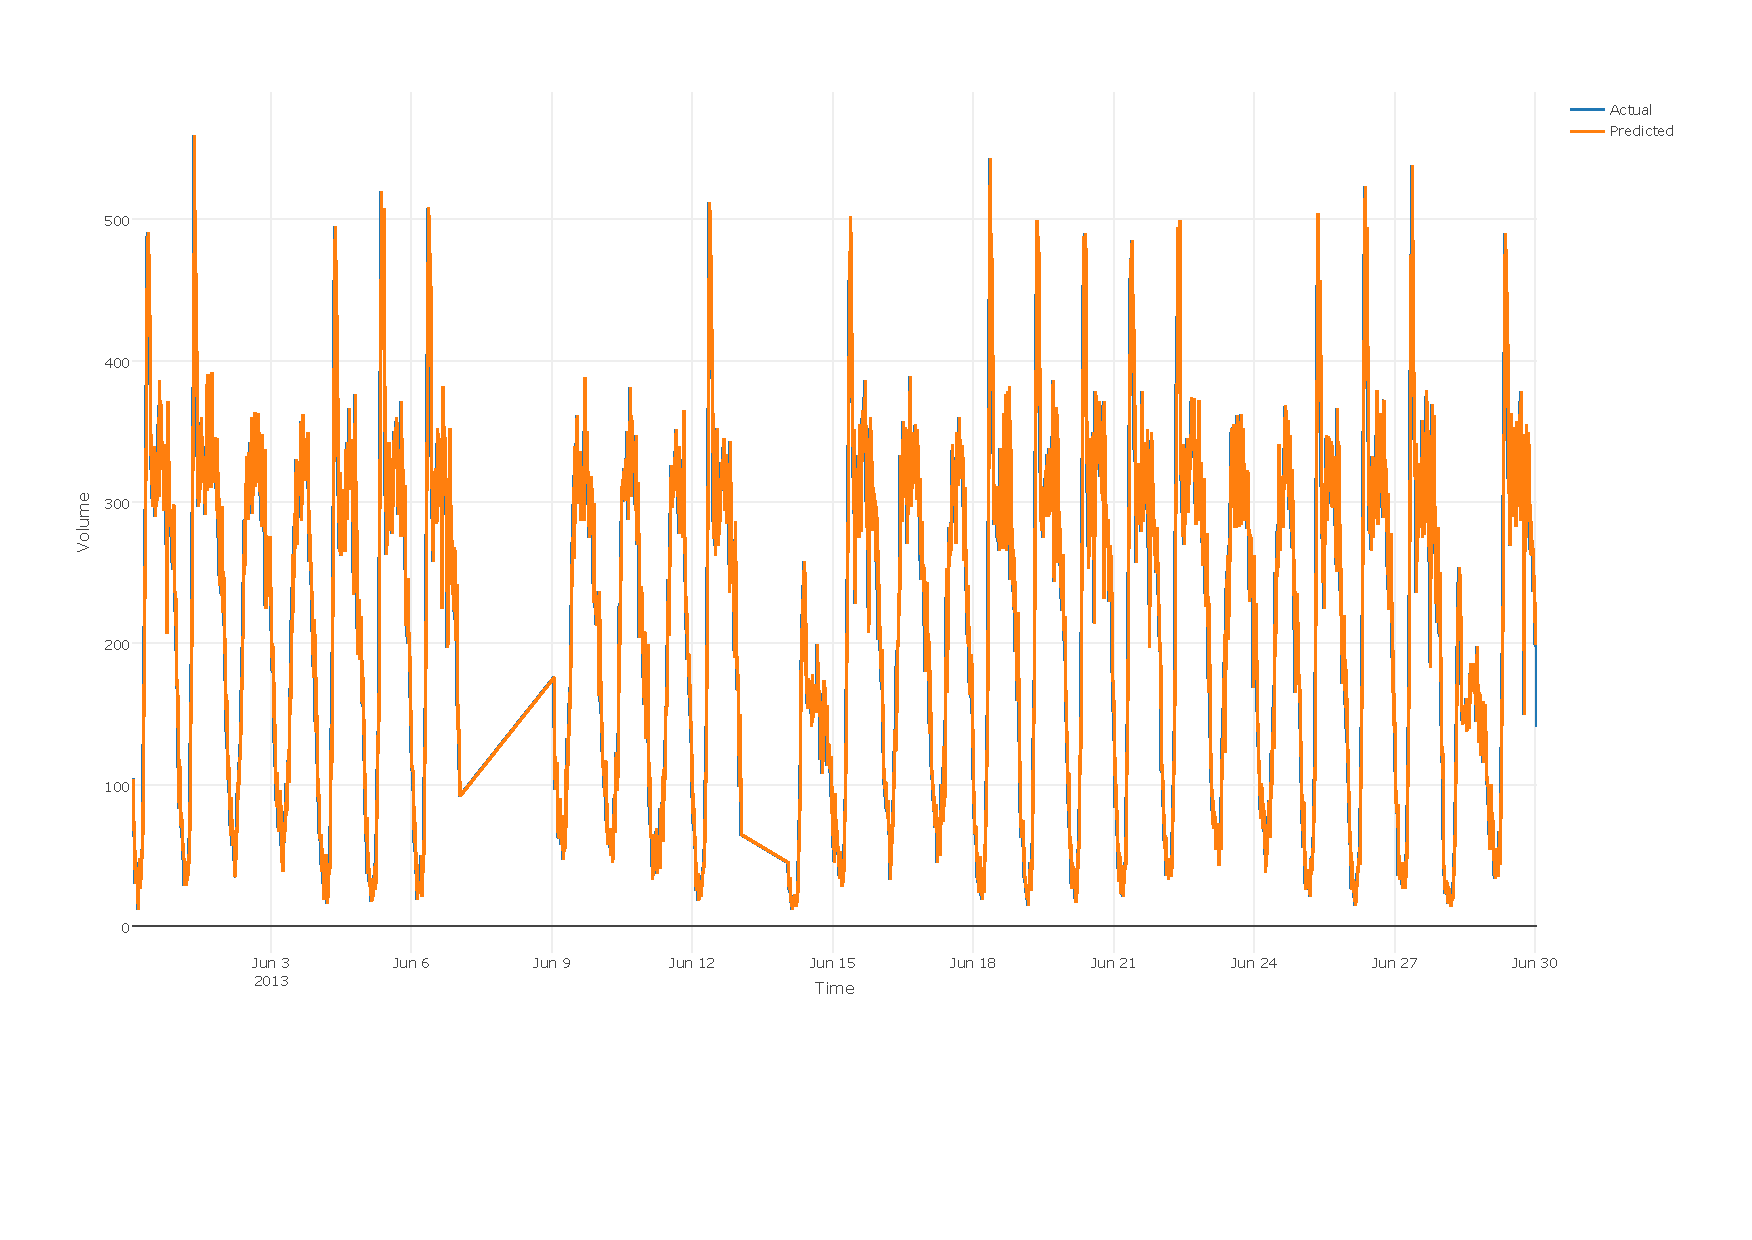
\includegraphics[width=0.7\textwidth]{Plots/naive1.pdf}
    \rule{35em}{0.5pt}
    \caption[Results of the Naive method]{Results of the Naive method, which is used as the baseline method.}
    \label{fig:baseline}
\end{figure}


Once the baseline is set, we used the comparing models to find out their performance. The results of
the comparing models are presented in figure \ref{fig:comparedModels}.


\begin{itemize}

\item \textbf{Linear regression}: We used a linear model for time series regression. The model was
created using the season component of the traffic volume time series data. The model
did not perform well, in fact its performance was the worst among all the models used in this
experiment.

\item \textbf{ARIMA}: After handling missing data, the Box-Cox transformation was done to stabilise the
variance. Then Using the Hyndman-Khandakar algorithm, the best ARIMA model was chosen. The selected
model was a seasonal ARIMA(2,0,5)(1,0,0)[96]. The model was fit using data from January to May 2012 with
frequency 96. Once the model was fit forecasts at steps 1 to 3 (15,30 and 45 minutes horizon) were
done in a recursive manner, that is after every forecast the model was refit using the newly available
observed data. The ARIMA model performed better than the baseline.

\item \textbf{Exponential smoothing}: For exponential smoothing, a state space model was used. This
model was a damped linear method with additive errors. Data preprocessing was done by handling missing
data through interpolation and then applying Box-Cox transformation to stabilise the variance. The
model used the same data used for the ARIMA model. The performance of the model was worse when compared
to the ARIMA model.

\item \textbf{Neural network autoregression}: A simple feedforward network with one hidden layer
was used. The lagged values of traffic volume time series were used as inputs to this network. A
38-20-1 neural network with 801 weights was used. Again for training purpose the same data that
was used for ARIMA and exponential smoothing methods were used. The performance of this model
was very good, better than the ARIMA model.

\item \textbf{K Nearest neighbour}: A neighbour based regression model was used, where the number
of nearest neighbours, k is set to 5. This value was selected by using both the autocorrelations and
cross validations. The distance measure was used to assign weights to each value in the local
neighbourhood.

\item \textbf{Support vector regression}: An epsilon-SVR with RBF kernel was used for this experiment.
The input data was standardised to mean 0 and variance 1.

\end{itemize}

\begin{figure}[h]
    \centering
    \subfloat[Linear Regression][Linear Regression]{
    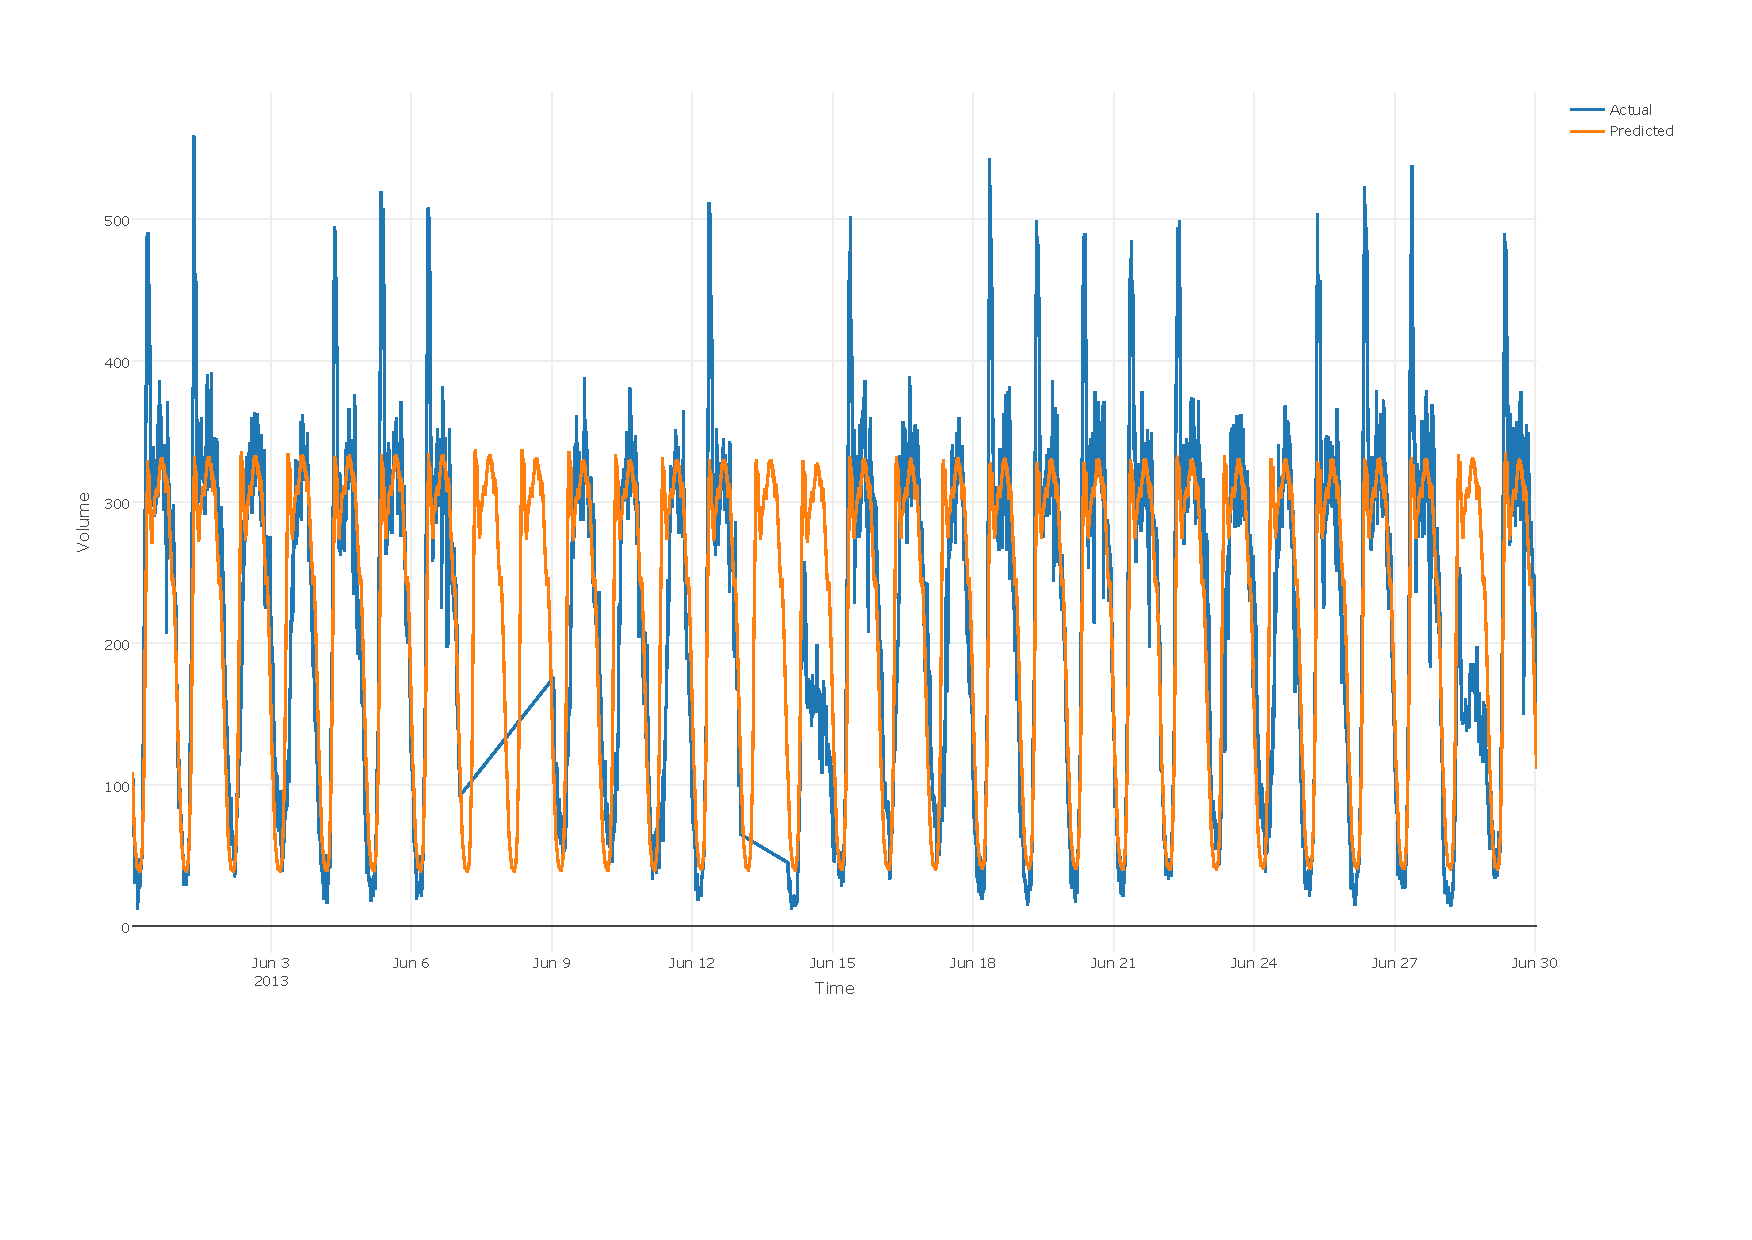
\includegraphics[width=0.4\textwidth]{Plots/linear1.pdf}
    \label{fig:lm1ActualPredicted}}
    \qquad
    \subfloat[ARIMA][ARIMA]{
    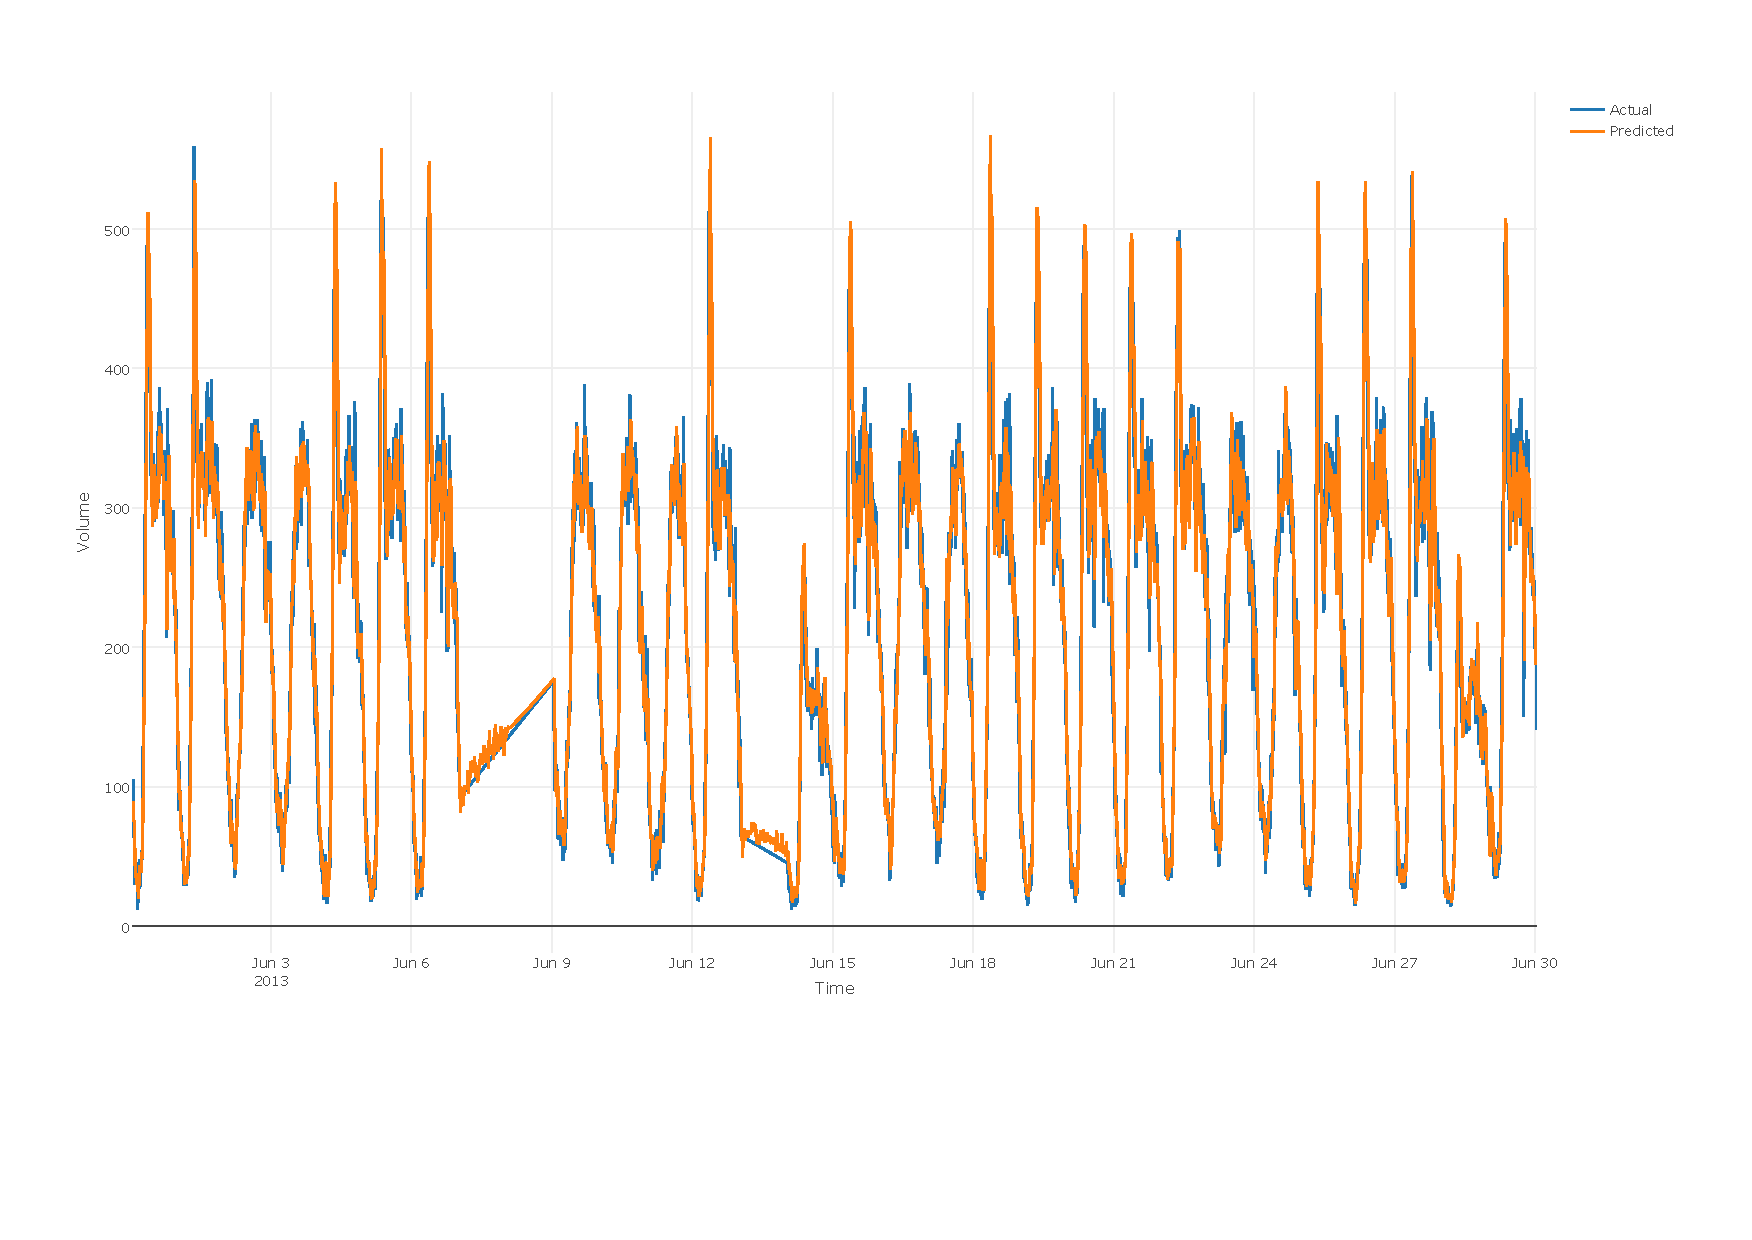
\includegraphics[width=0.4\textwidth]{Plots/arima1.pdf}
    \label{fig:arima1ActualPredicted}}

    \subfloat[Exponential smoothing state space model][Exponential smoothing state space model]{
    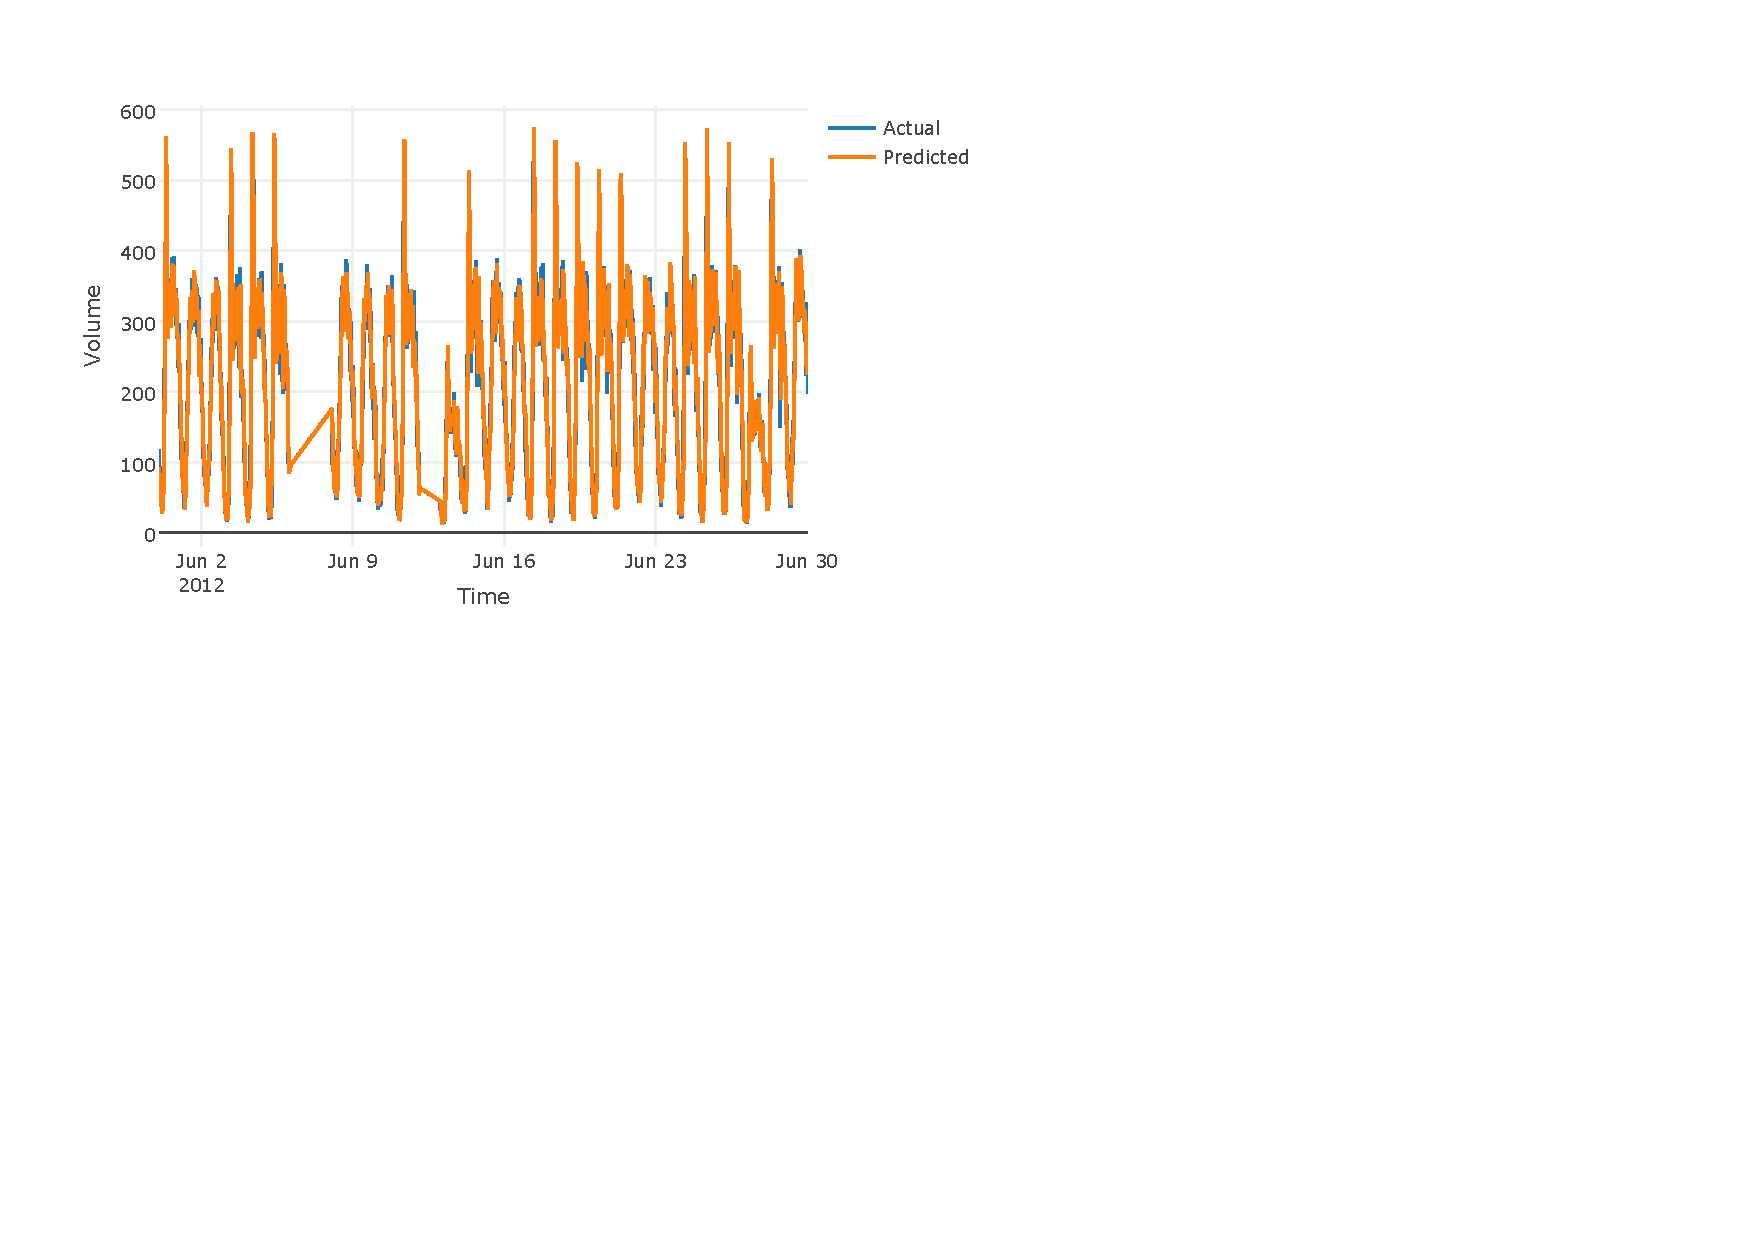
\includegraphics[width=0.4\textwidth]{Plots/ets1.pdf}
    \label{fig:ets1ActualPredicted}}
    \qquad
    \subfloat[Neural Network AutoRegression][Neural Network AutoRegression]{
    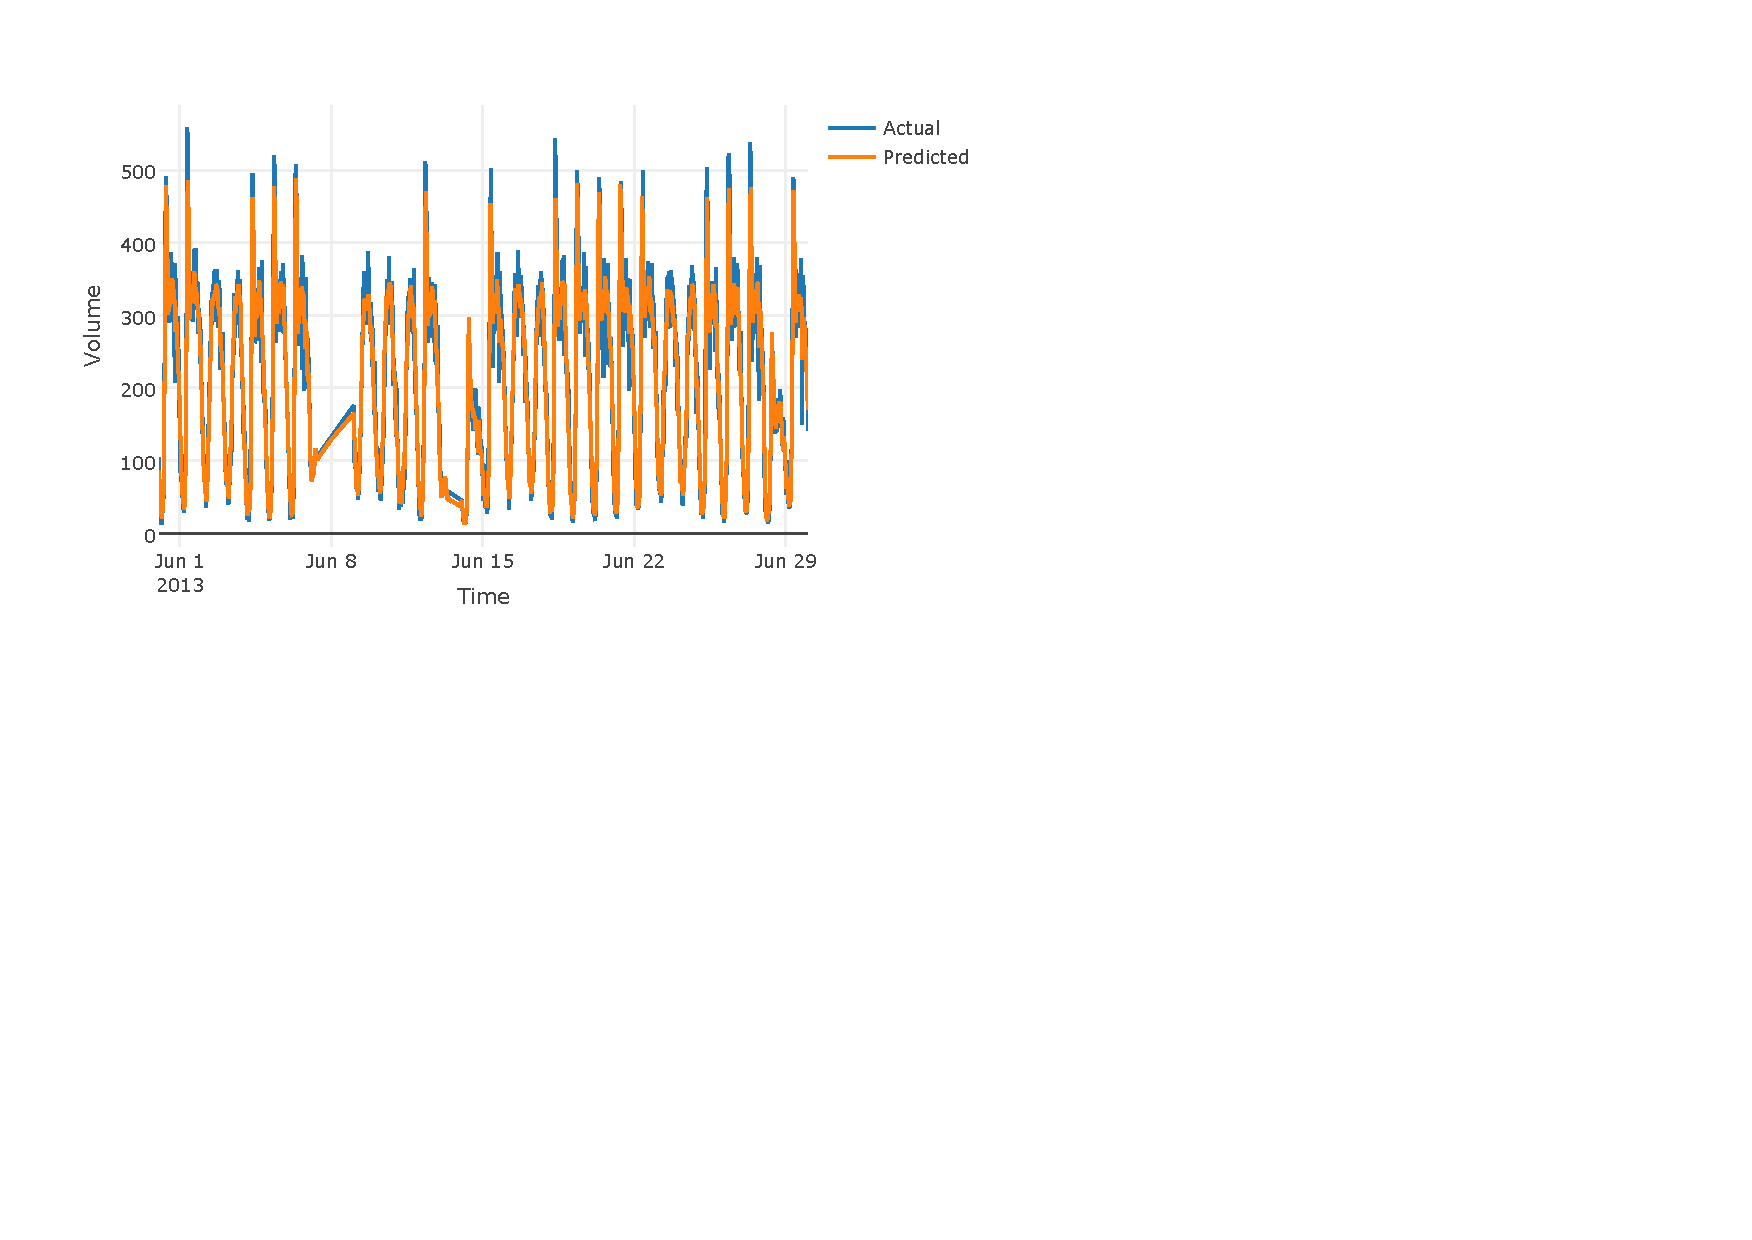
\includegraphics[width=0.4\textwidth]{Plots/nnetar1.pdf}
    \label{fig:nnetar1ActualPredicted}}

    \subfloat[K-Nearest Neighbour][K-Nearest Neighbour]{
    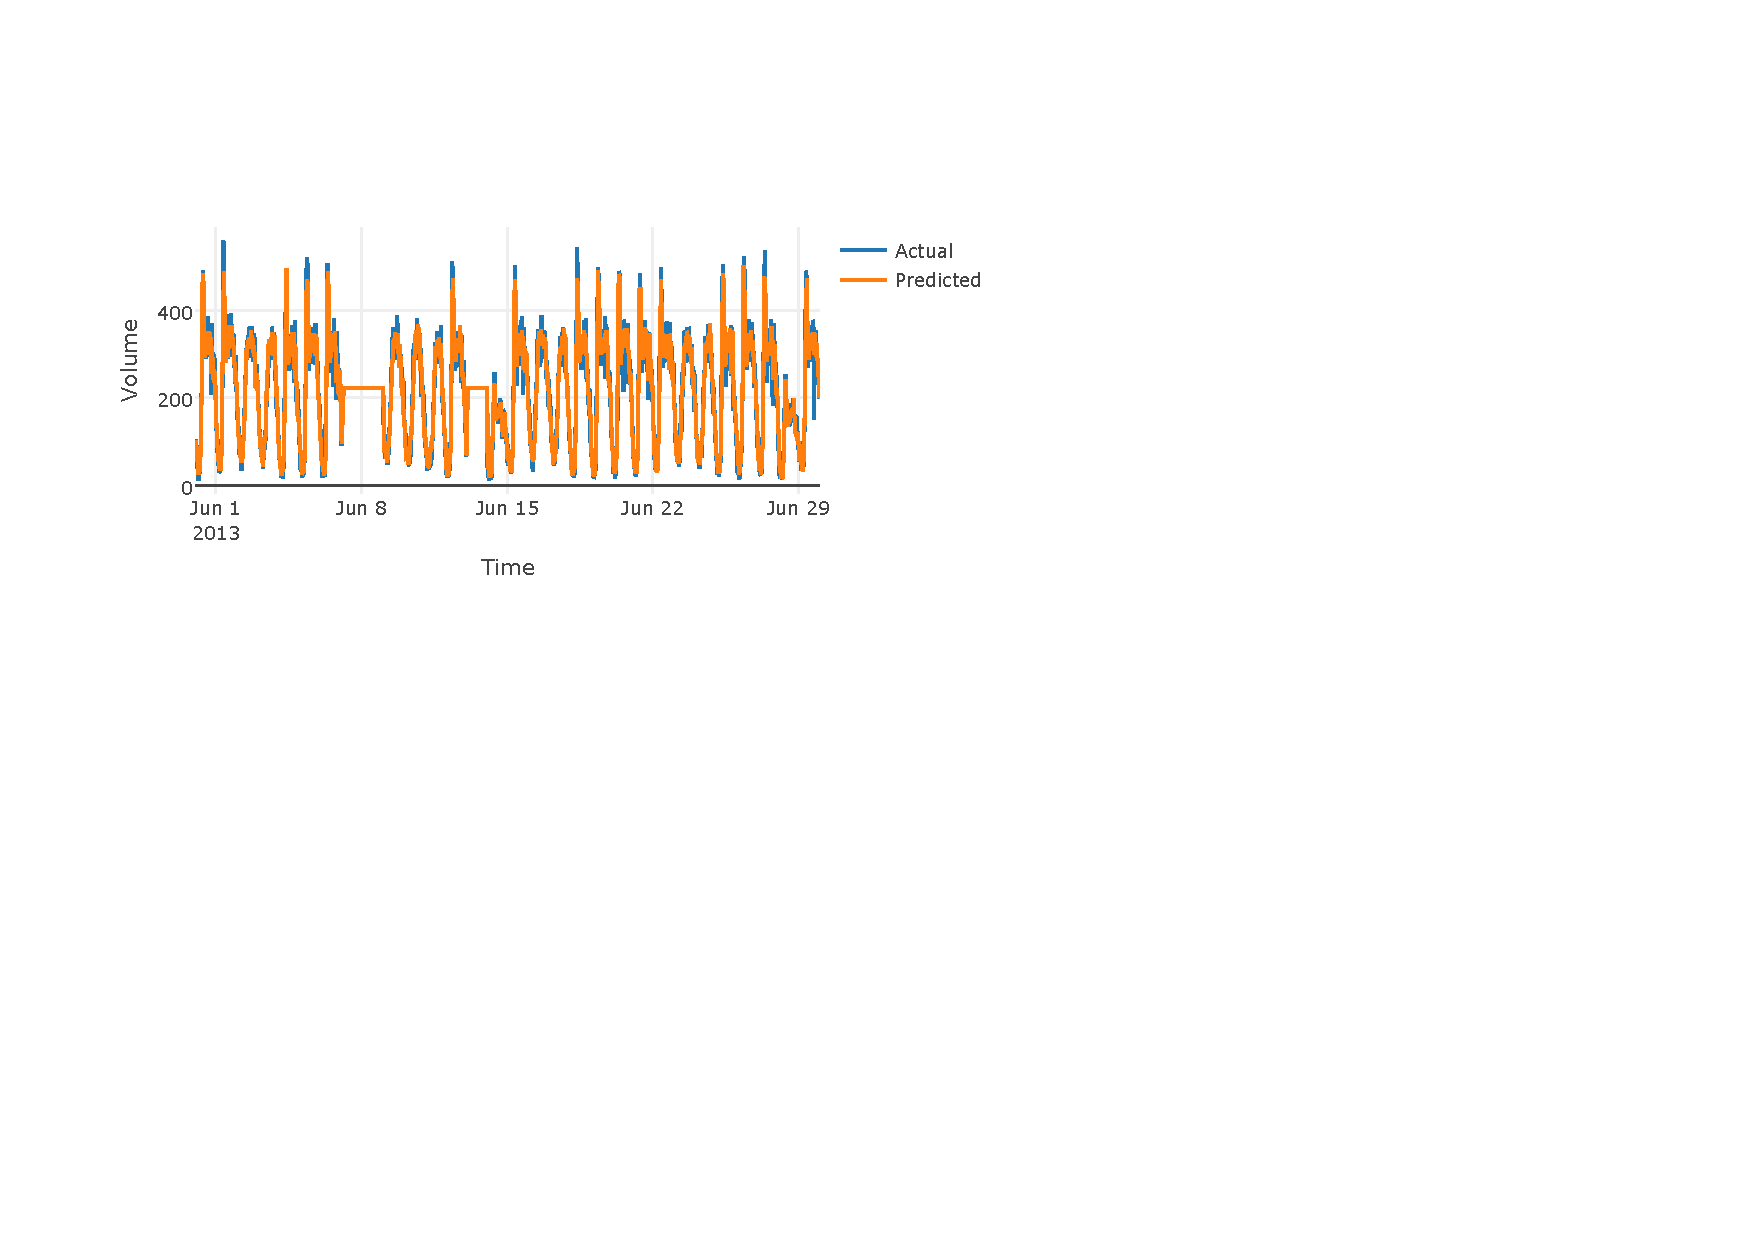
\includegraphics[width=0.4\textwidth]{Plots/knn1.pdf}
    \label{fig:knn1ActualPredicted}}
    \qquad
    \subfloat[Support Vector Regression][Support Vector Regression]{
    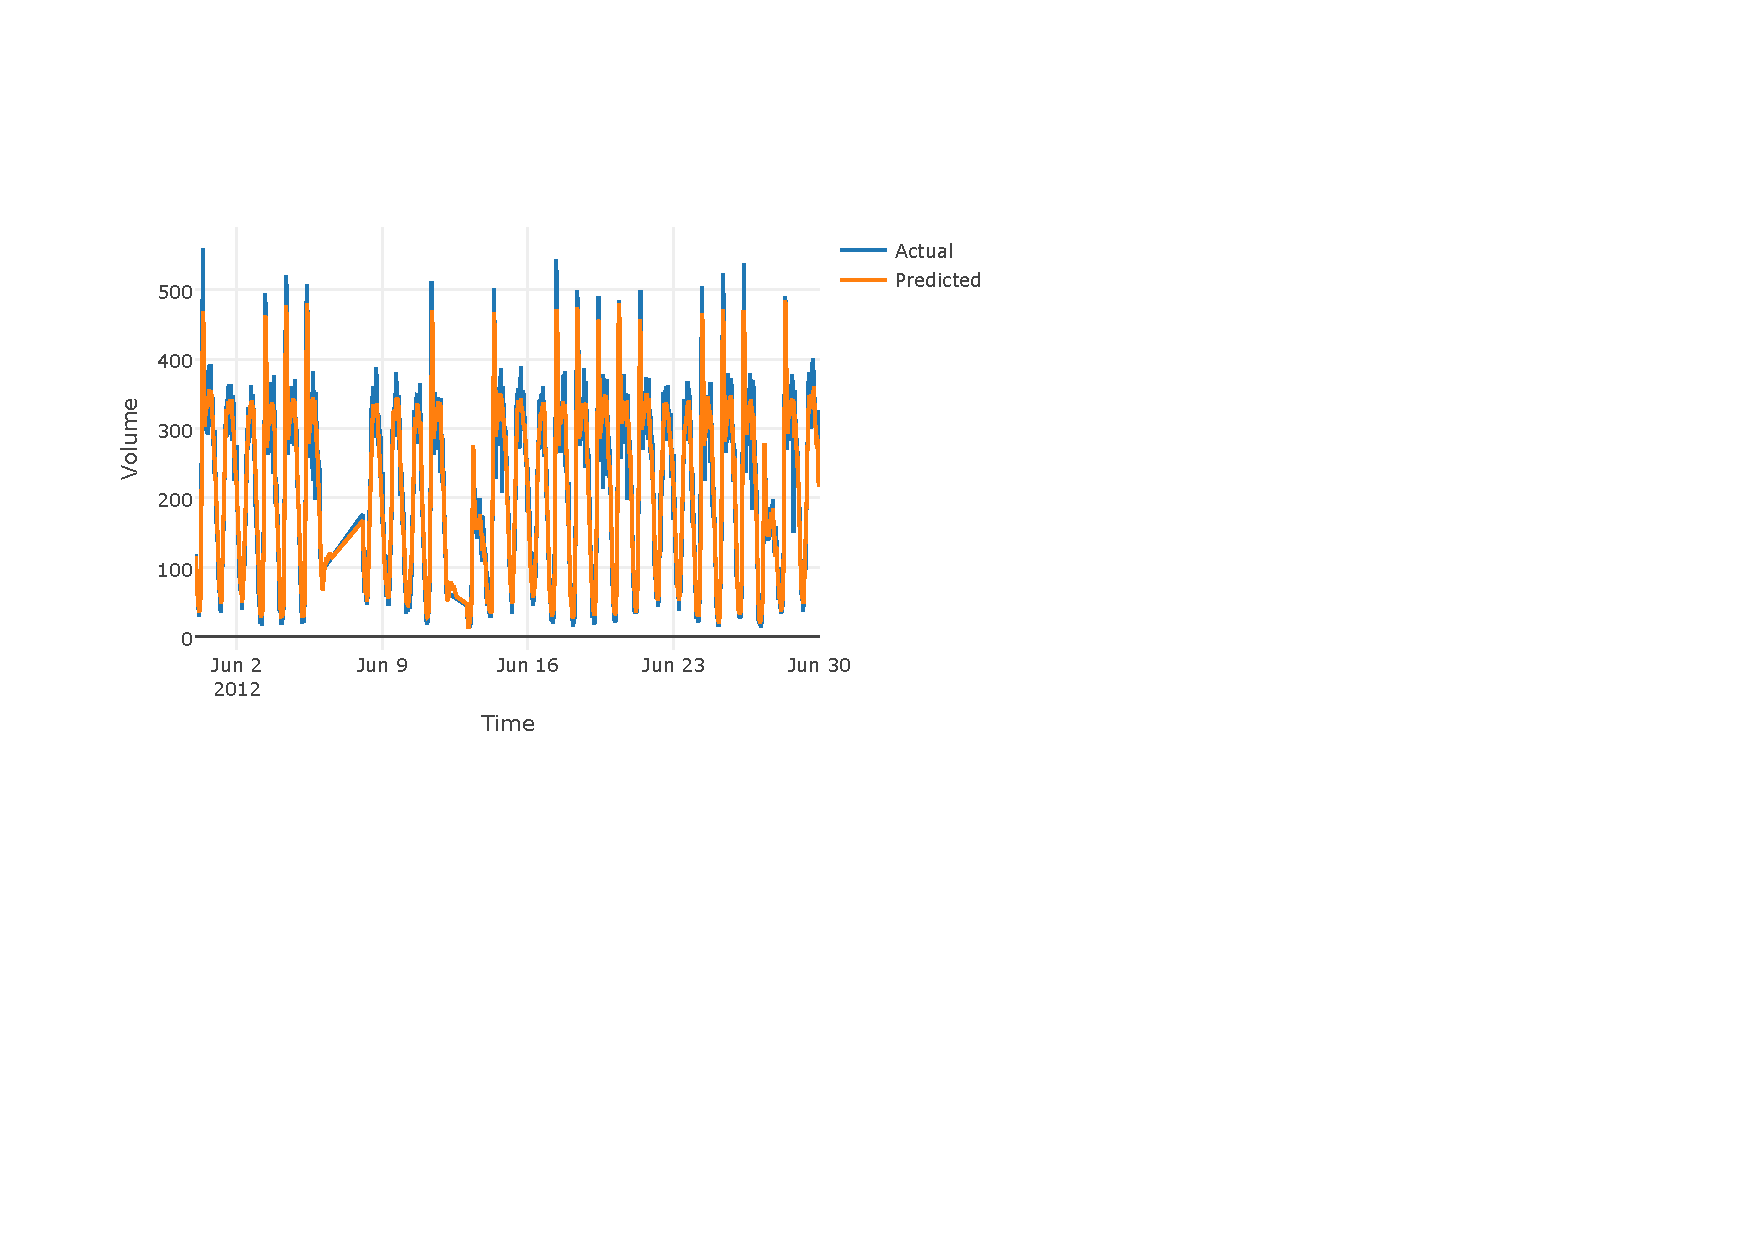
\includegraphics[width=0.4\textwidth]{Plots/svm1.pdf}
    \label{fig:svm1ActualPredicted}}

    \caption[Actual vs Predictions, using currently popular methods]{Actual vs Predictions -
    naive, linear regression, ARIMA, simple feed forward neural network with one hidden layer, exponential
    smoothing using state space model, k-nearest neighbour and support vector regression.
    The models were trained on traffic data from one homogeneous road segment. The plots show the
    actual vs predictions (15 mins) for the month of June 2012.}
    \label{fig:comparedModels}
\end{figure}

\section{Deep neural network models}
The experiment details of the three used models are presented below.
We used these models on two sets of data. First dataset is from a single location as mentioned earlier.
The second dataset contains volume data from the location of interest and its neighbourhood locations.
The input data used were standardised to mean zero and variance 1. We used various setting for
length of the sequence, number of hidden layers and number of units in those layers and optimisation
algorithms used for optimising the gradients. We present the final settings of these models below.
The results of these models are shown in the figure \ref{fig:deepNNModels}.

\begin{itemize}

\item \textbf{Simple RNN}: The simple RNN used was a fully connected RNN where the output was fed
back to the input is used. For univariate modelling, that is using data from a single location and
make predictions for that location, the RNN model with 2 hidden layers with 100 units in each
layer was used. To avoid overfitting a dropout of 10\% was used at both the hidden layers. The weights
were initialised randomly using the uniform distribution. A linear activation function was used
in the output layer. The loss function used for training was the mean squared error. Finally for
optimising gradients, the RMSprop algorithm, which was proposed by Geoff Hinton, was used.
The RMSprop is an adaptive learning rate algorithm. The input data was a set of sequences, where
each sequence was created with 50 time steps. We trained the model for 30 epochs.
For multivariate modelling three hidden layers with number of units [100,200,200] were used.
The input data consisted of the traffic volume data from the location of interest along with data
from 10 other locations in the neighbourhood. The weight initialisations, optimising algorithm and
error functions were same as the univariate model.

\item \textbf{GRU}: Gated Recurrent Unit is a simple version of LSTM and was recently proposed.
Similar to the simple RNN modelling, we used GRU to model both univariate and multivariate datasets.
For univariate model, the network consisted of two hidden layers with 100 units in each of them.
We used the RMSprop algorithm for gradient optimastion. The number of epochs used was 30. Simlilar to
the RNN network input data was a set of sequences, where each sequence was created with 50 time steps.
For multivariate modelling we used three hidden layers with number of units [100,200,200].

\item \textbf{LSTM}: An LSTM model was also implemented for modelling both univariate and multivariate
traffic volume datasets, similar to the above RNN and GRU networks. For univariate modelling number
of combinations of hidden layers and units in those were used. The final univariate model consisted
of two hidden layers with 100 and 200 units in them. The output layer had an linear acivation function.
Different sequence lengths were used and a final length of 50 was selected. For optimisation purpose
we tried both the RMSprop and Adaptive Moment Estimation (ADAM) algorithms. We found that the
ADAM algorithm outperformed the RMSprop. We trained the netowrk for 20 epochs. For multivariate
modelling we used three hidden layer with [100,200,200] units. Again we compared the RMSprop and ADAM
optimisation algorithms and found the later outperformed the former again.

\end{itemize}


\begin{figure}[h]
    \centering

    \subfloat[LSTM - single location][LSTM - single location]{
    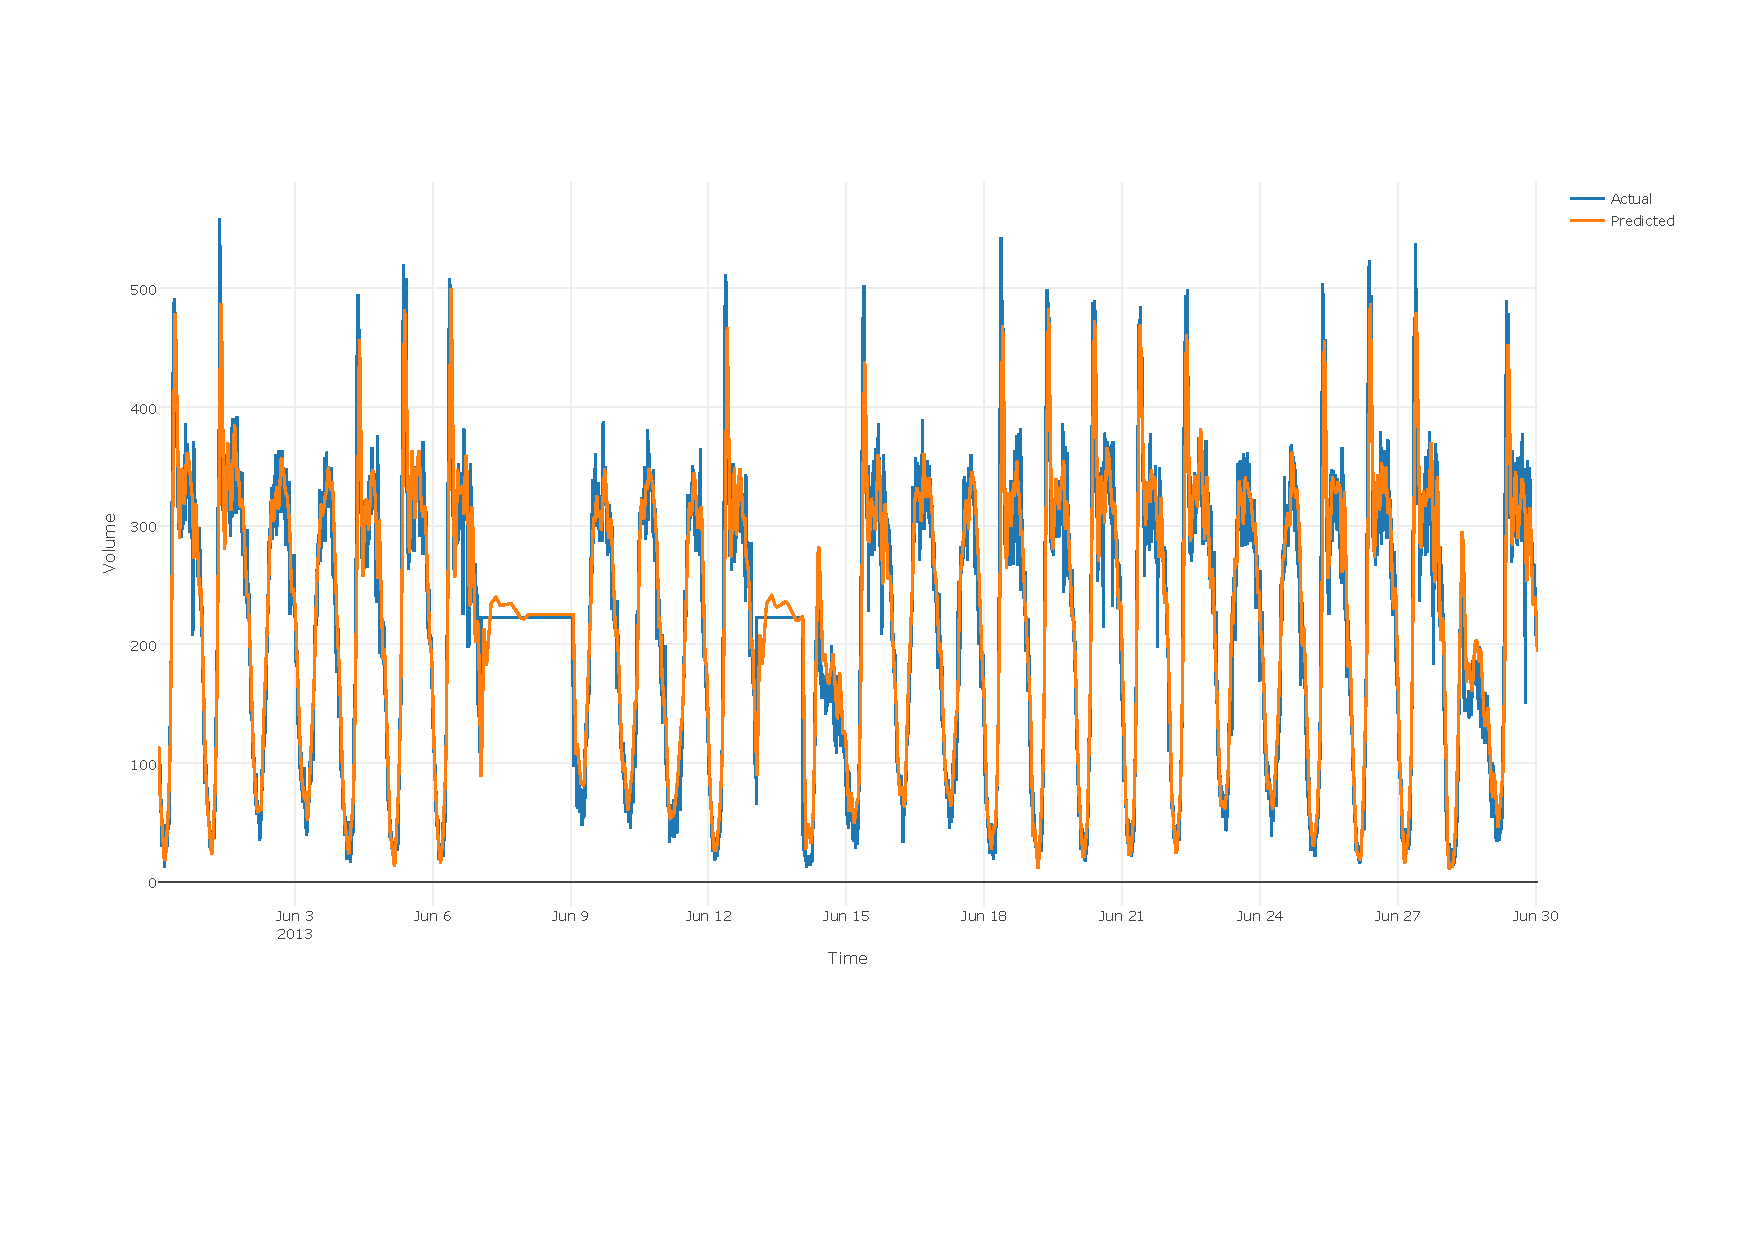
\includegraphics[width=0.4\textwidth]{Plots/lstm-single1.pdf}
    \label{fig:LSTMActualPredicted1}}
    \qquad
    \subfloat[GRU - single location][GRU - single location]{
    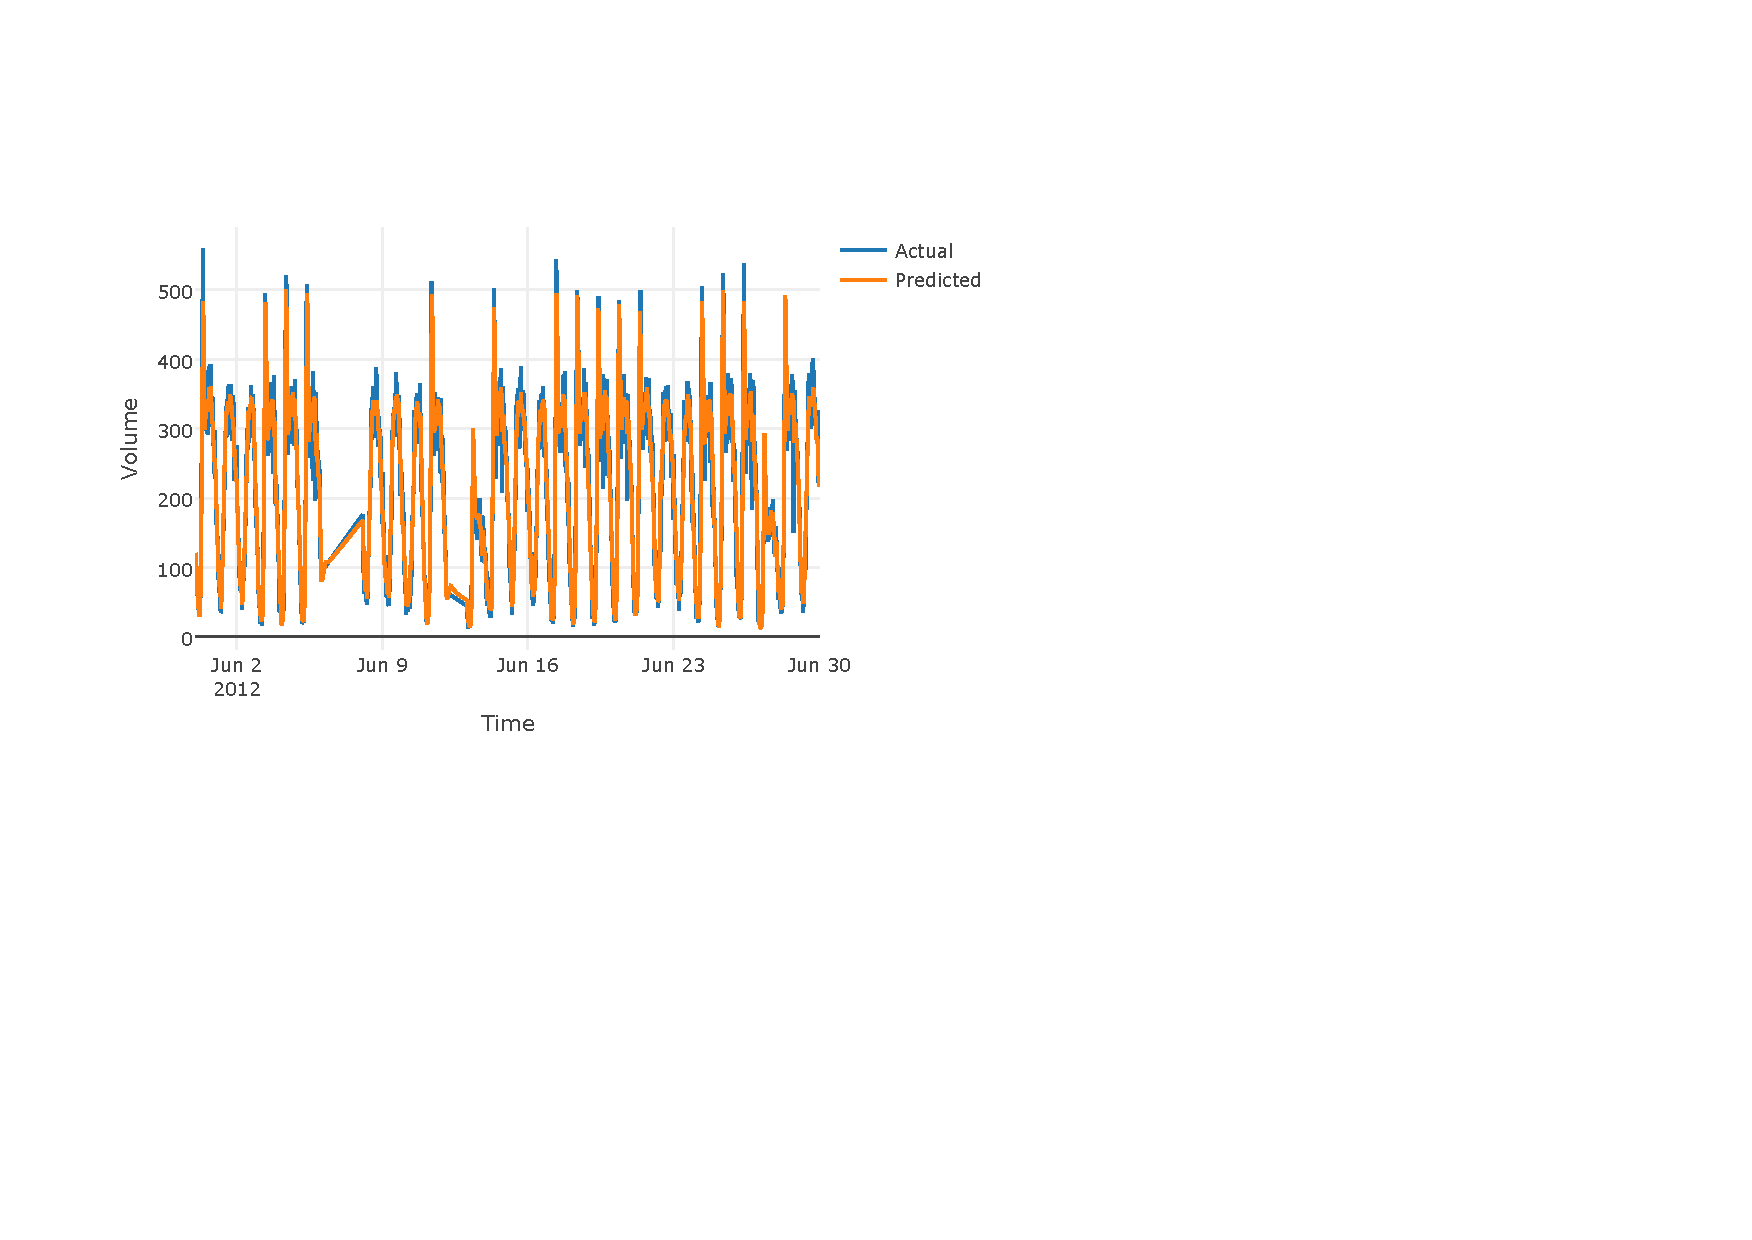
\includegraphics[width=0.4\textwidth]{Plots/gru-single1.pdf}
    \label{fig:GRUActualPredicted1}}

    \subfloat[RNN - single location][RNN - single location]{
    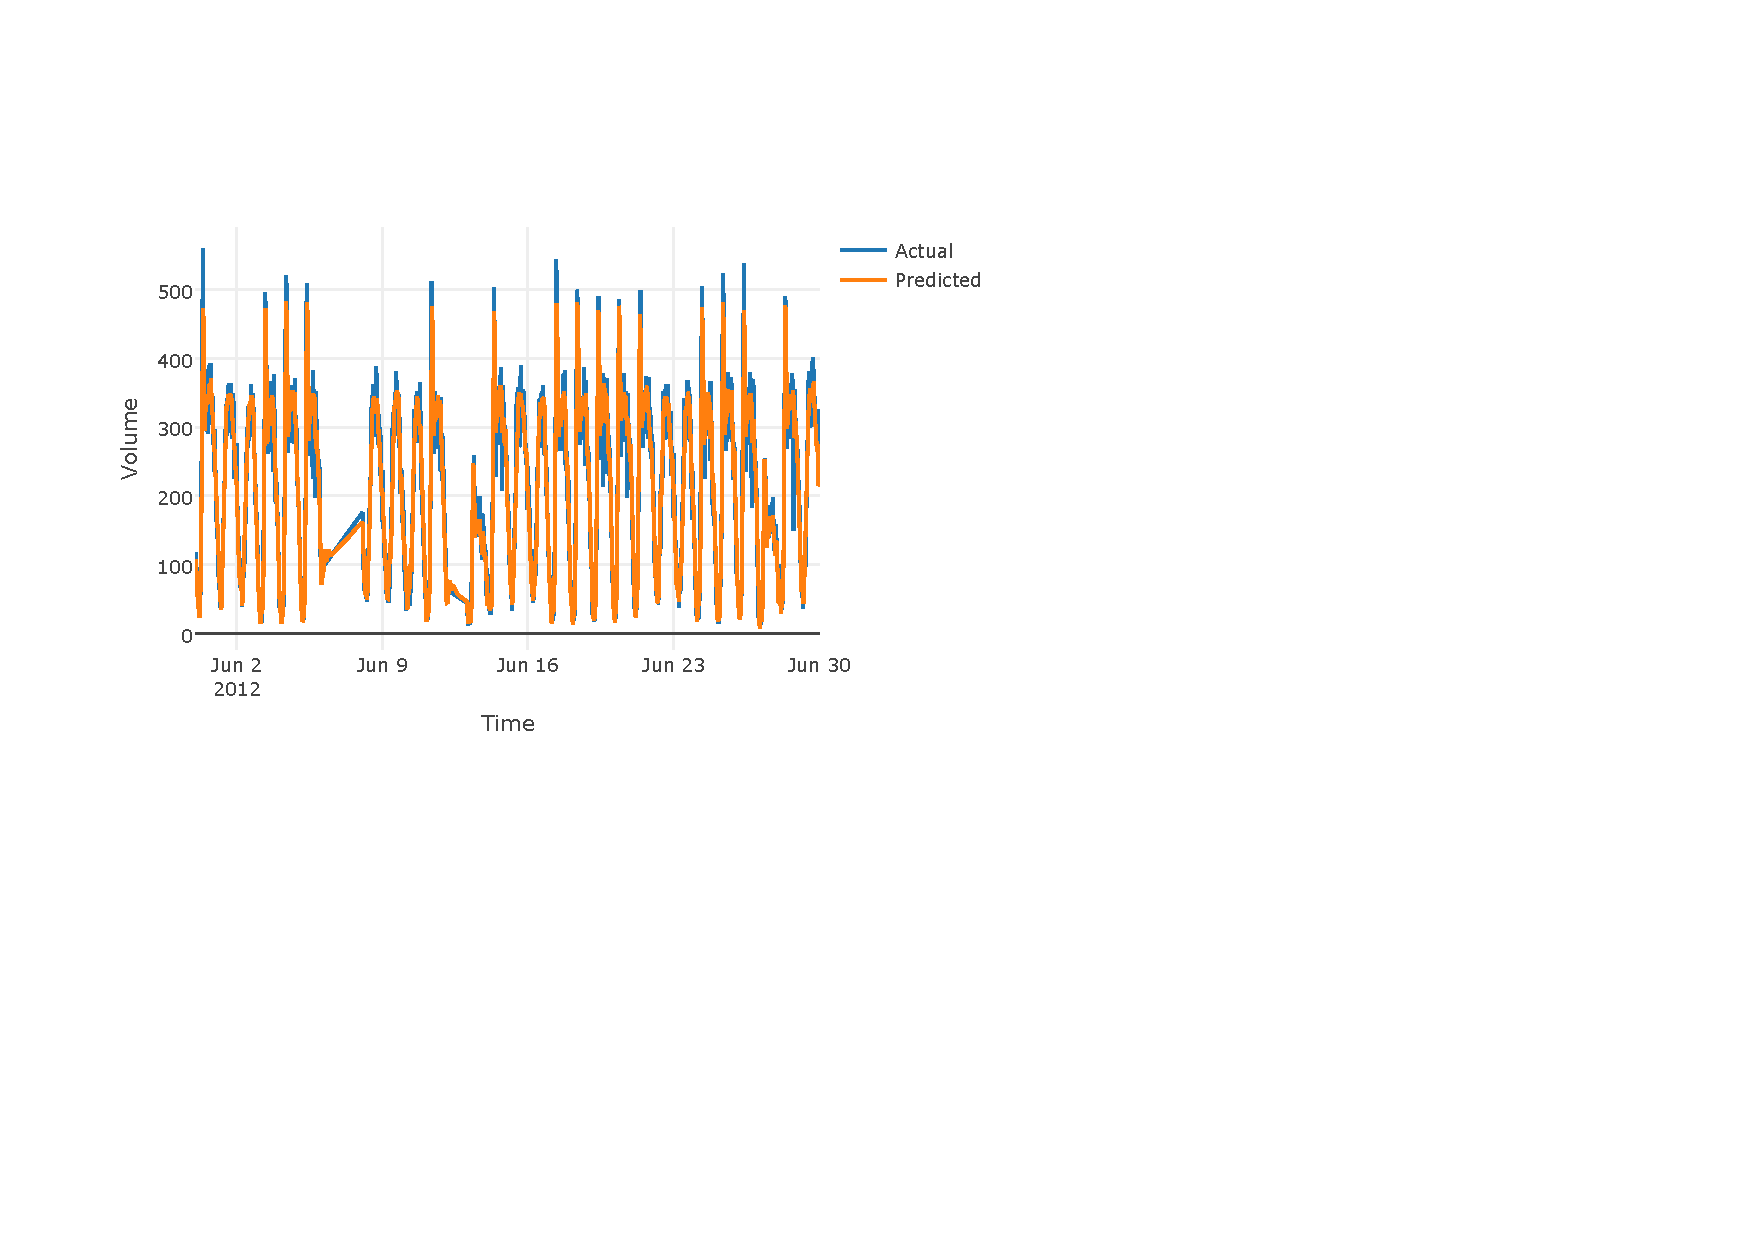
\includegraphics[width=0.4\textwidth]{Plots/rnn-single1.pdf}
    \label{fig:RNNActualPredicted1}}

    \subfloat[LSTM - multiple locations][LSTM - multiple locations]{
    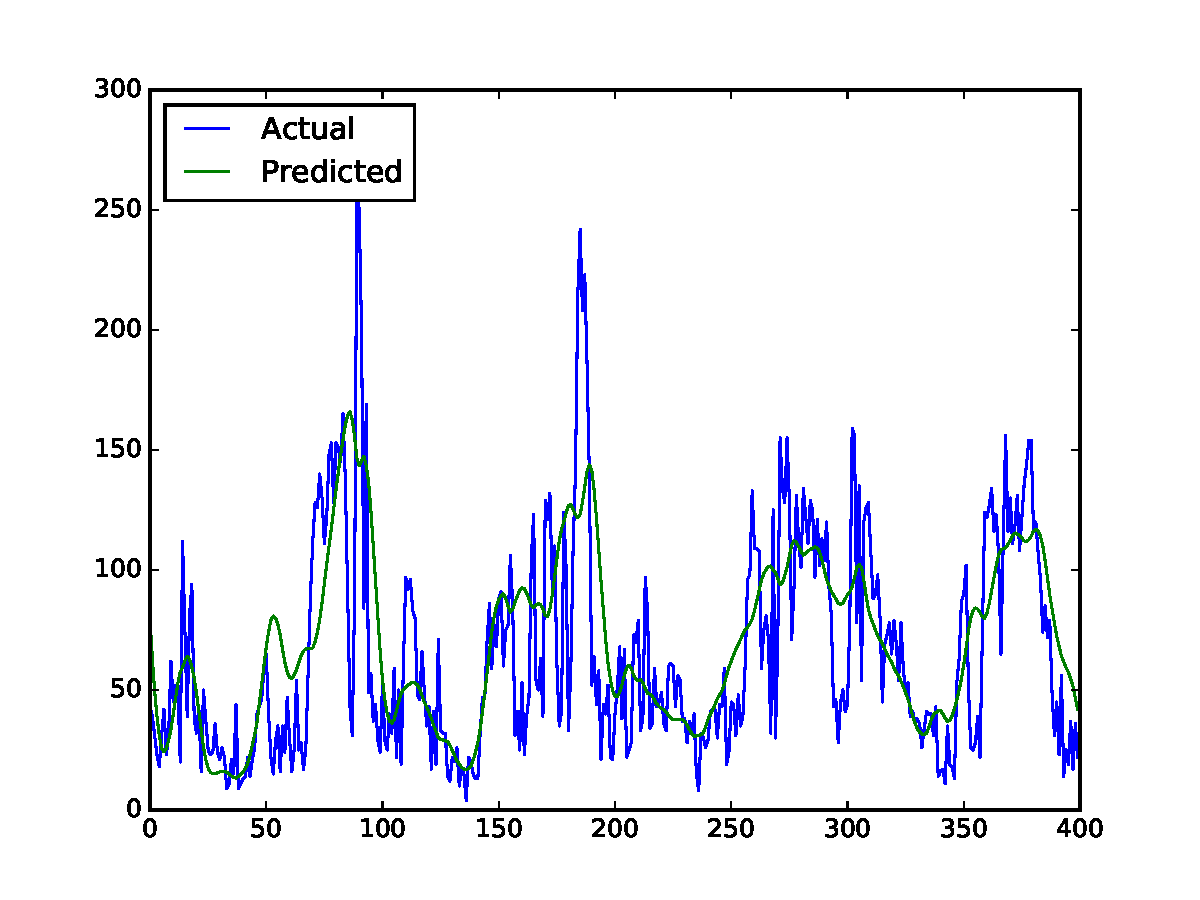
\includegraphics[width=0.4\textwidth]{Plots/lstm-multi1.pdf}
    \label{fig:LSTMMultiActualPredicted1}}
    \qquad
    \subfloat[GRU - multiple locations][GRU - multiple locations]{
    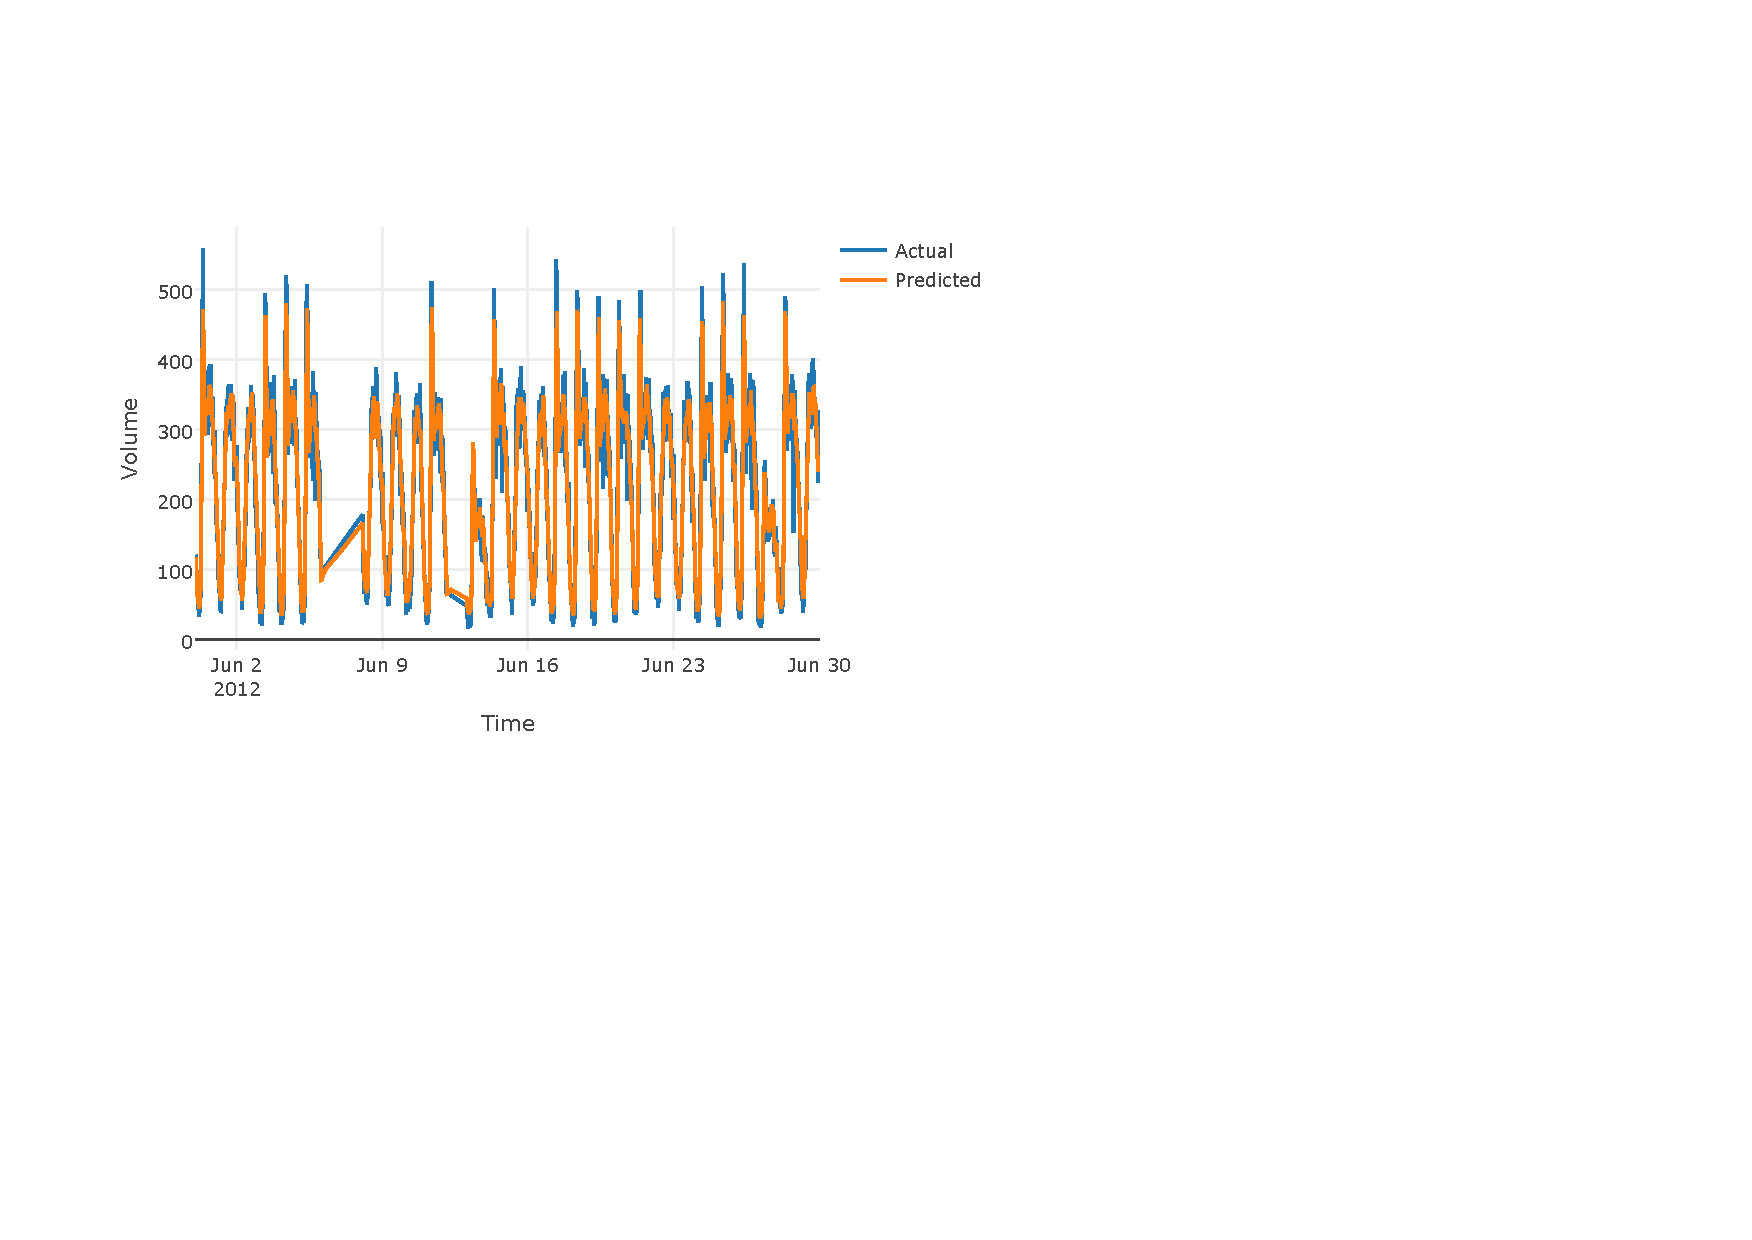
\includegraphics[width=0.4\textwidth]{Plots/gru-multi1.pdf}
    \label{fig:GRUMultiActualPredicted1}}

    \subfloat[RNN - multiple locations][RNN - multiple locations]{
    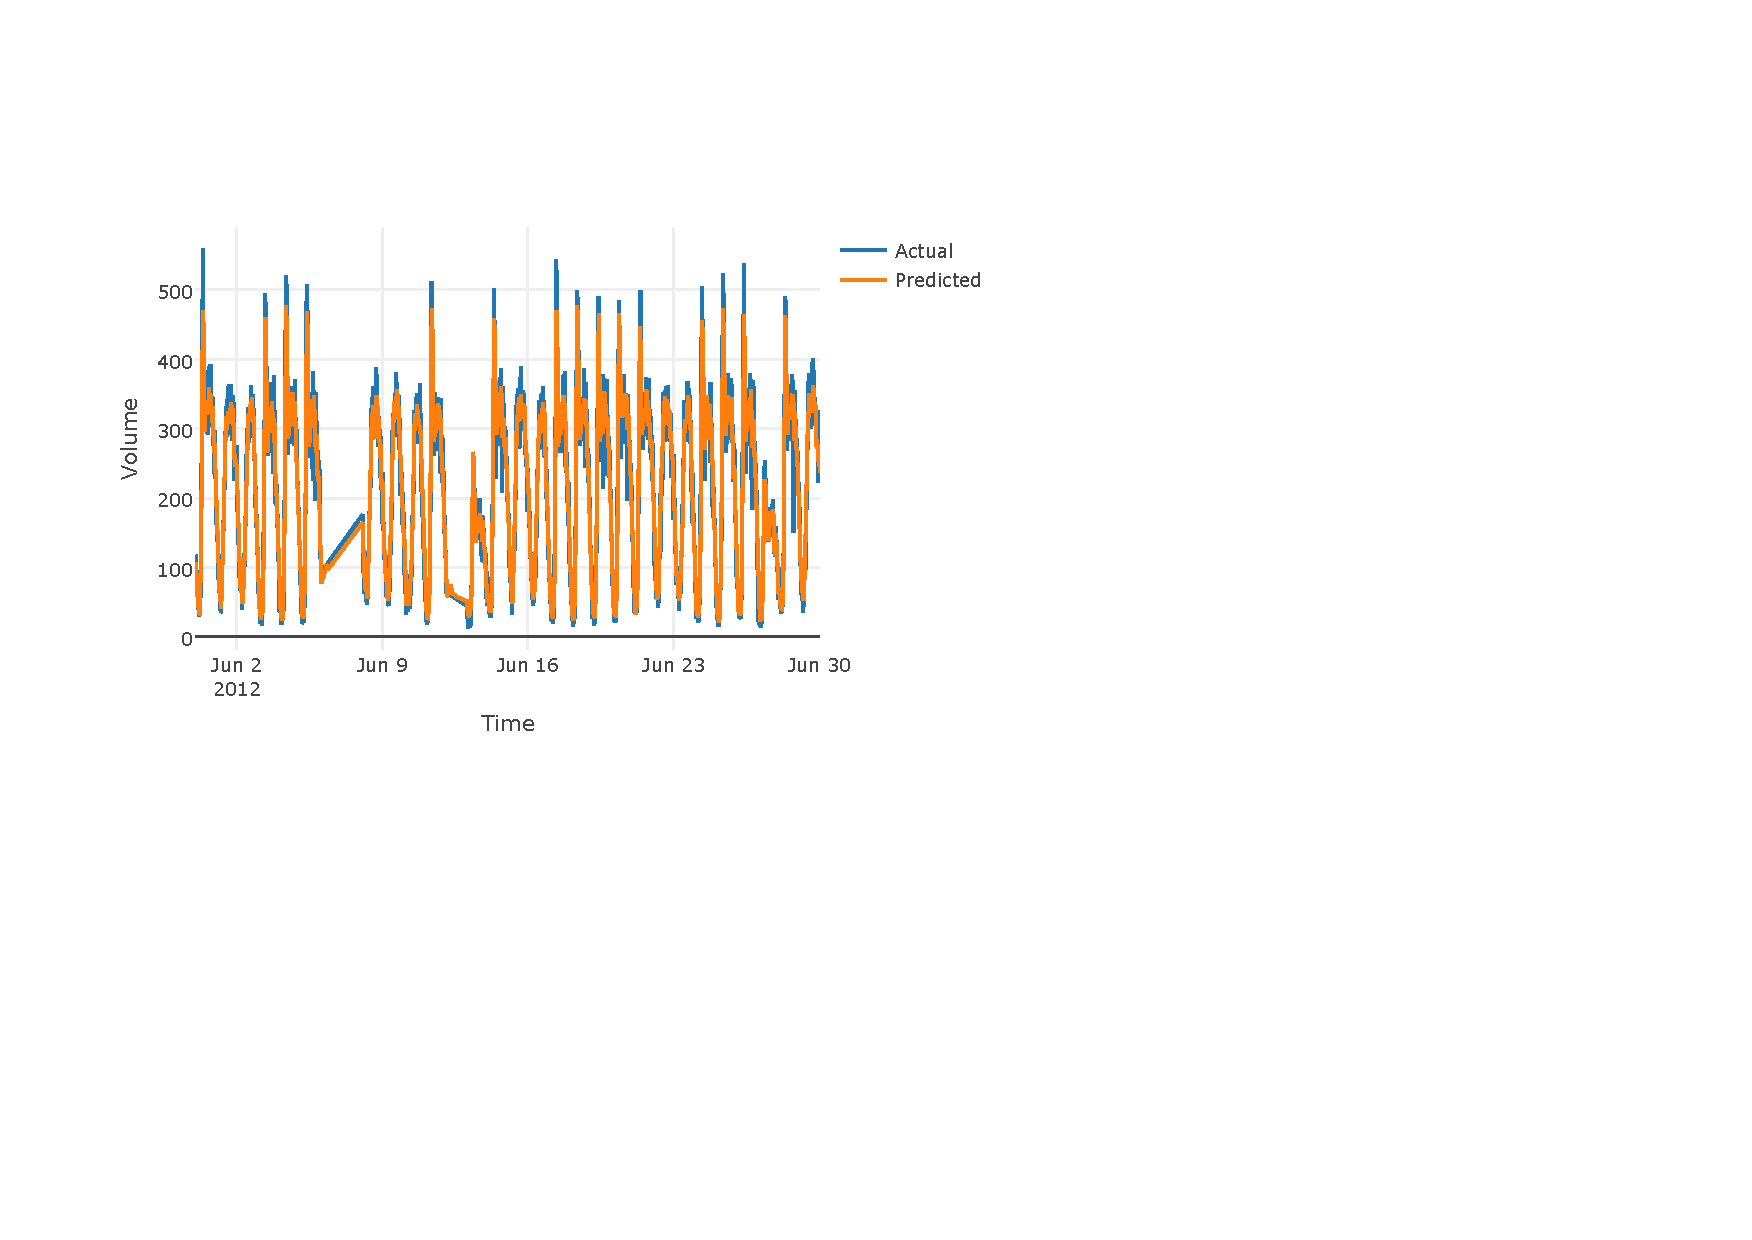
\includegraphics[width=0.4\textwidth]{Plots/rnn-multi1.pdf}
    \label{fig:RNNMultiActualPredicted1}}

    \caption[Actual vs Predictions, using deep networks]{Actual vs Predictions - using three deep
    neural networks (LSTM, GRU and Simple RNN). The top three are results for the single homogeneous
    road segment when using data from that location only while the bottom three are results for the
    single homogeneous road segment when data from neighbouring locations (\ref{fig:ExperimentRegion})
    were also used . The plots show the actual vs predictions (15 mins) for the month of June 2012.}
    \label{fig:deepNNModels}
\end{figure}

\section{Comparisons}
For model comparison we used three accuracy measures - mean absolute error (MAE), root mean squared
error (RMSE) and mean absolute percentage error (MAPE). In below sections we briefly describe
the accuracy measures.

For defining the accuracy measures let us denote $x_{i}$ be the $i^{th}$ observation and
$\hat{x}_{i}$ be the prediction of $x_{i}$.

\textbf{Scale-dependent errors}
The prediction error is simply given by $e_{i} = x_{i} - \hat{x}_{i}$, which is in the same scale
as of the original data. So accuracy measures that depend on $e_{i}$ are scale dependent and can
not be used across multiple series on different scales. The two most used scale-dependent
accuracy measures are mean absolute error and root mean squared error defined as below

    \begin{equation}
        MAE = mean(\abs{e_{i}})
    \end{equation}
    \begin{equation}
        RMSE = \sqrt{mean(e^{2}_{i})}
    \end{equation}

MAE is easy to understand and popular in usage when using a single dataset.

\textbf{Percentage errors}
Percentage errors are scale-independent and thus used across multiple datasets on different
scales. The percentage error is given by $p_{i} = 100*e_{i}/x_{i}$. The most commonly used
percentage measure is Mean Absolute Percentage Error (MAPE) which is given by the below formula
    \begin{equation}
        MAPE = mean(\abs{p_{i}})
    \end{equation}

There are however few shortcomings of the MAPE, for instance when $x_{i}$ is 0 or very large.
Another shortcoming is that they put heavier penalty on negative error values than positive error
values.

In table \ref{table:accuracyScores}, the accuracies are presented in terms of the above mentioned
error measures for the methods presented in this expriment. The error measurea are presented for
the predictions for 1 step-ahead (15 minutes), 2 steps-ahead (30 minutes) and 3-steps ahead (45 minutes).
The linear regression has the worst performance among all the methods including the baseline naive
method. All other methods performed better than the baseline. For both one step-ahead and multi
step-ahead predictions, deep LSTM netork with multivariate modelling had the best performance.

\begin{table}
    \begin{tabular}{c}
        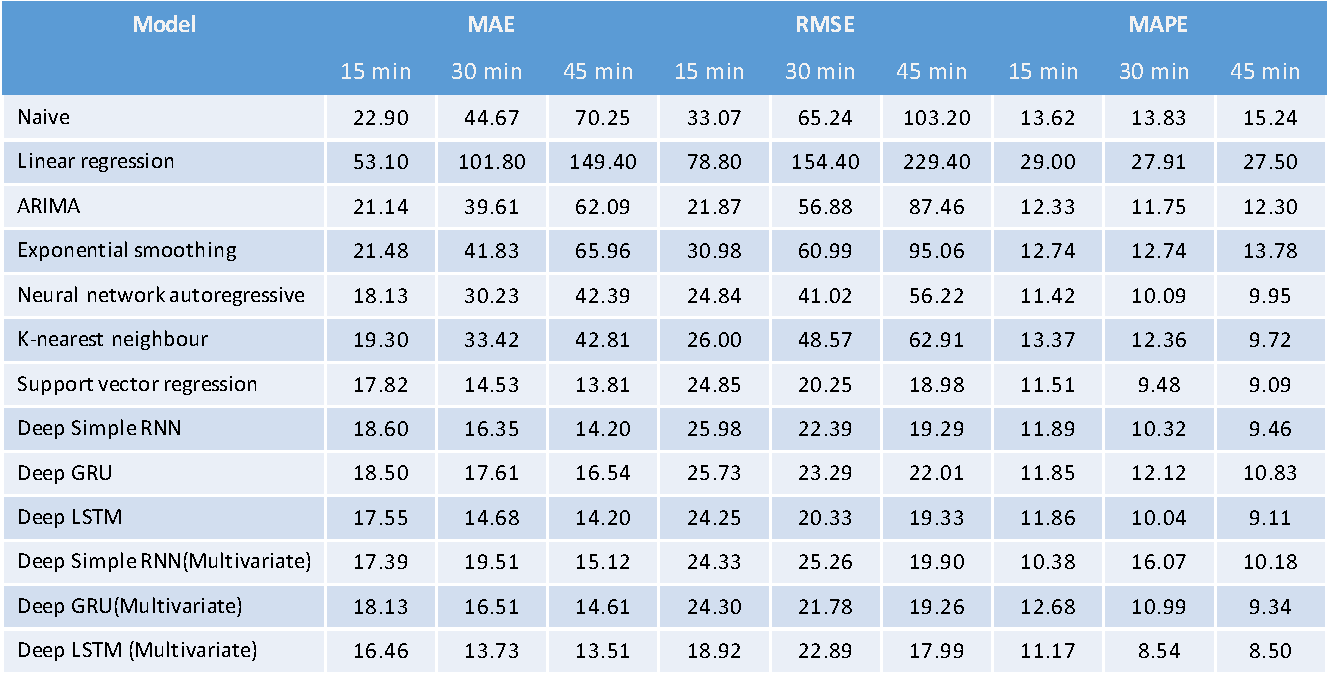
\includegraphics[width=\textwidth,height=\textheight,keepaspectratio]{Figures/errors-table.pdf}
    \end{tabular}
    \caption[Model comparisons]{Accuracy measures for the evaluated models. The scores are
    calculated for prediction horizon of 15-minutes and 30-minutes. Mean 15-minutes traffic
    volume is 224.1}
    \label{table:accuracyScores}
\end{table}

For all these experiments we used a home computer with Intel i7-4770 CPU, 16GB RAM, GeForce GTX 960
GPU. The operating system used was Ubuntu 14.04 and for data processing and modelling we used R and
Python languages. The training time of all the above mentioned models (except Naive)  are shown in
the figure \ref{fig:trainingTime}. However not all of the algorithms were used optimised to reduce
the training time, so the figures could vary in small amounts.

\begin{figure}[htbp]
    \centering
    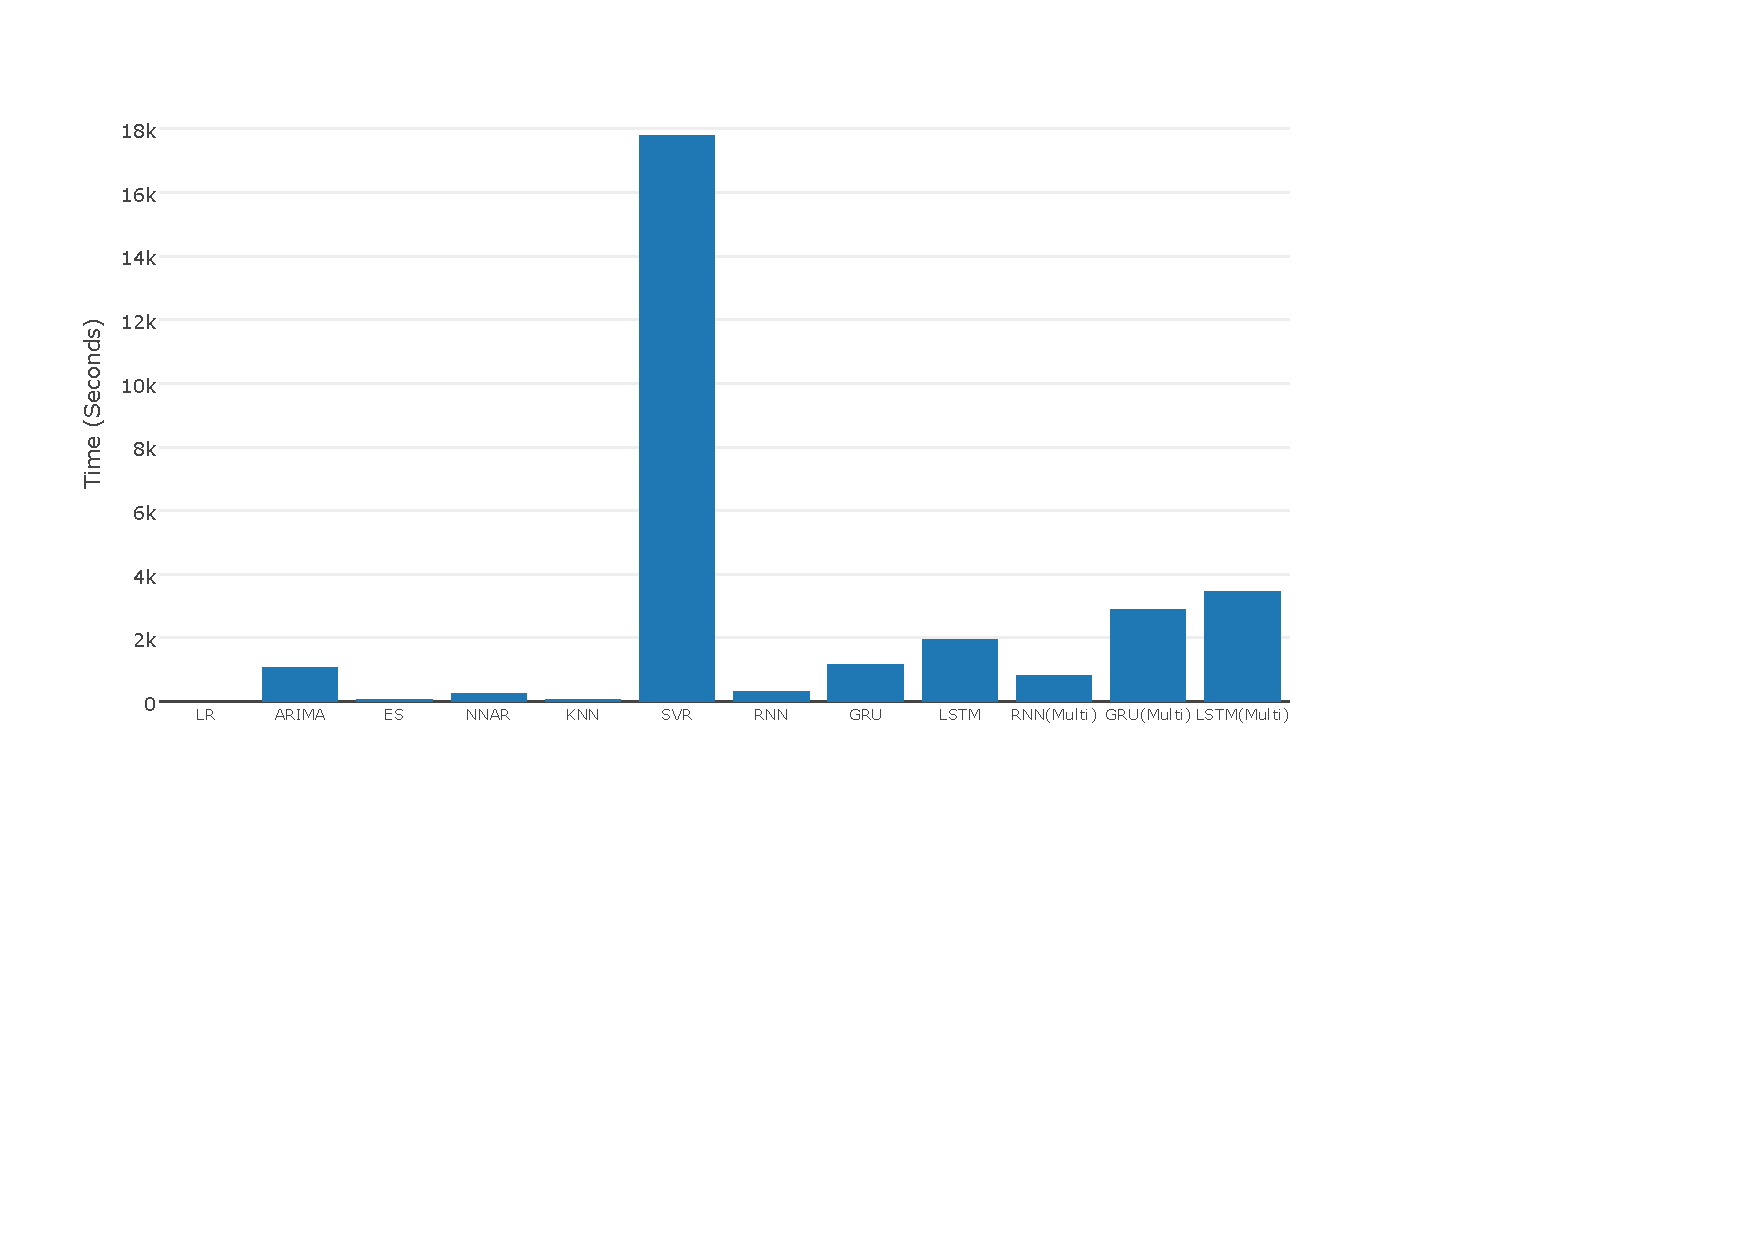
\includegraphics[width=0.7\textwidth]{Plots/training-time.pdf}
    \rule{35em}{0.5pt}
    \caption[Comparison of training time of the models]{Comparison of training time of the models}
    \label{fig:trainingTime}
\end{figure}

In this chapter we presented the results of our expeiments in short term traffic prediction using
several meodels. We compared the results and found that the performance of deep neural networks
outperform all the exisitng methods.